\documentclass[../structure.tex]{subfiles}
%\usepackage{../mypkg}
\begin{document}
\chapter{Background}
The human brain, which is the focus of our work in this thesis, is the central organ of the human nervous system. It is made up of two main components, namely, gray 	     		matter and white matter. Researchers have discerned a great deal about gray and white matter and distinct brain regions through autopsies and imaging techniques. The study 		of the human brain in diseased states or under conditions associated with brain damage have resulted in major insights into this complex organ.

\section{Brain Anatomy :Fiber Pathways}

	 \textbf{White matter} areas in the central nervous system are made up of myelinated axons, also known as tracts or fiber pathways \cite{Blumenfeld2010}. Fiber pathway is composed of bundles which connect various gray matter areas of the brain together and carry nerve impulses between neurons. Myelin acts as an insulator allowing electrical signals to jump rather than course through axons, increasing the speed of transmission of all nerve signals through a phenomenon known as saltatory conduction \cite{Klein2008}.
%	\\Long thought to be passive tissue, white matter affects learning and brain functions, modulates the distribution of action potentials, and acts as a relay and coordinator of communication between different brain regions \cite{Fields2008}.
	
	The human brain consists of the following tracts on both the left and right sides:


	\begin{figure}[h!]
	\centering
	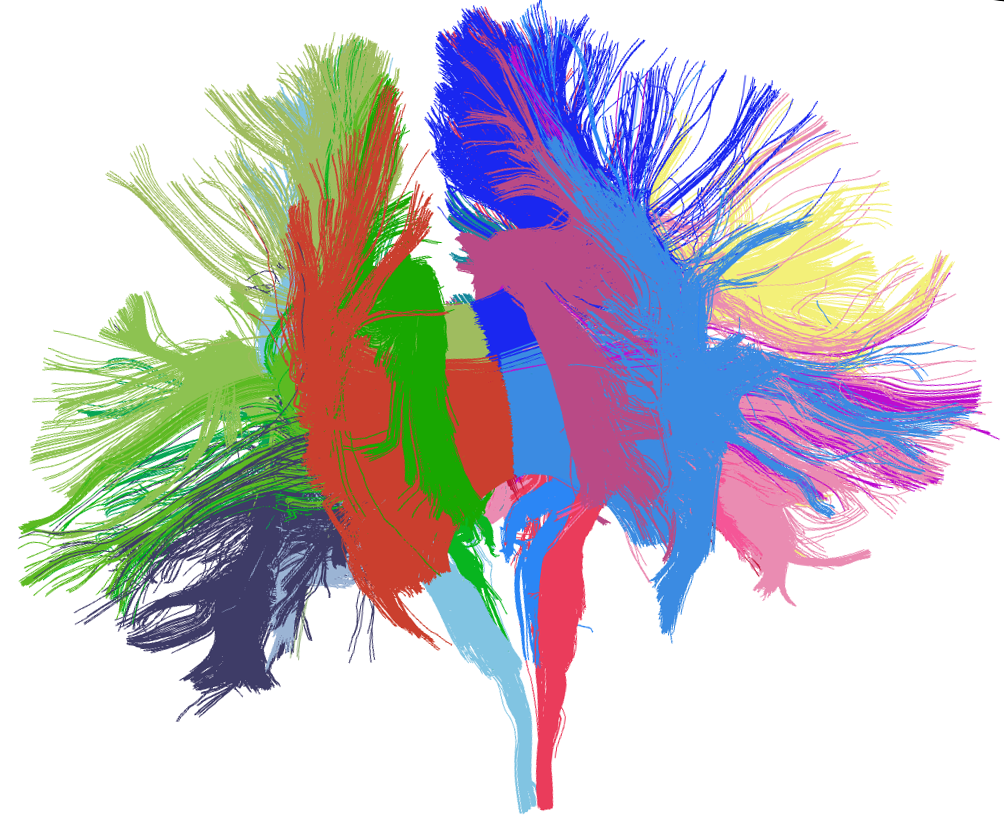
\includegraphics[scale=0.4]{000_all_brain}
	\captionsetup{justification=centering}
	\caption{The Human Brain Fiber Pathway}
	\label{fig:all_brain}
	\end{figure}
	
	\textbf{Thalamic Radiation (ATR)} \\
	ATR is a nerve fiber bundle connects the anterior nuclear group of the thalamus and the midline nuclear group of the thalamus with the frontal lobe through the anterior thalamic peduncle, the anterior limb of the internal capsule and other parts of the cerebral white matter \cite{Washington1994}\cite{Grimm2018}. Abnormalities in ATR have a possible link with cognitive abnormalities and symptoms in schizophrenia\cite{Mamah2010}.	\\
		

	\textbf{Corpus Callosum (CC)} \\
	CC is one of the largest transverse fibre and white matter tract in the brain that links the cerebral cortex of the left and the right cerebral hemisphere. CC is divided into an anterior portion called \textit{genu} , \textit{rostrum} that continuous with the lamina terminalis, posterior structure known as \textit{splenium} and in between its anterior and posterior portions is the \textit{trunk/body}.\\


		\textbf{Cingulum (Cing)}  \\
		CC is a collection of white matter fibres that connects portions of the parietal lobe, cingulate gyrus and prefrontal cortex with the parahippocampal gyrus and adjacent structures of the temporal lobe that always pass through the cingulum bundle  \cite{Washington1994}. It is described as a C shaped structure from various brain images that wraps around the frontal lobe to the temporal lobe above the corpus callosum. Posterior cingulate and anterior cingulate are two pimary parts of the cingulate cortex that are related to cognitive functions and emotion,  especially apathy and depression respectively \cite{JaredTanner2010}.\\
		
		
	\textbf{Corticospinal Tract (CST)} \\	
		CST plays an important role in cortical control of spinal cord activity. It is a major tract for motor function. The CST originates from secondary motor area, the parietal cortex, and the primary motor cortex. CST estimation and 3D visualization can be performed using diffusion tensor tractography, a technique derived from DTI \cite{Seo2013}.\\
		
		
		\textbf{Fornix (Fornix)} \\		
	Fornix, a discrete white matter tract bundle located on the medical aspects of the cerebral hemispheres is critical for normal cognitive functioning. It carries signals from the hippocampus to the hypothalamus which begins in the hippocampus on each side of the brain. Fornex can be identified and segmented by using diffusion tesnor imaging. Functionally relevant alteraions in forniceal integirty in heath and disease state can be identified using a technique called quantitative fiber tracking \cite{Thomas2011}.\\

	
		\textbf{Inferior Fronto-occipital Fasciculus (IFOF)} \\		
		IFOF is the one of the first association fiber systems to be recognized in the human brain \cite{Wu2016}. It passes through a depth of temporal lobe and insula, connecting occipital cortex, temporo-basal areas, and superior parietal lobe to the frontal lobe \cite{PDD2015} . \\

				
		\textbf{Inferior Longitudinal Fasciculus (ILF)}\\		
		ILF is an associative white matter pathway that connects the occipital and temporal-occipital areas of the brain to the anterior temporal areas.  Sudden disruption of the ILF by neurologic insult is mainly associated with  neuropsychological impairments of visual cognition such as visual agnosia, prosopagnosia, and alexia \cite{Herbet2018}. The ILF is in direct contact with few other association tracts namely, the uncinate fasciculus, the inferior fronto-occipital fasciculus (IFOF), the long and posterior/vertical segments of the arcuate fasciculus and the vertical occipital fasciculus of Wernicke.\\

		

		\textbf{Superior Longitudinal Fasciculus (SLF)}\\			
		SLF is a fiber pathway in the cerebral white matter that connect temporo-parietal language regions to ipsilateral frontal and opercular areas \cite{Madhavan2014}. It comprises three subcomponents namely, SLF I, II, and III linking the parietal lobe association cortices with the frontal lobe. The arcuate fasciculus (AF) were viewed as synonymous, by contrast, appears to be separate and distinct from the SLF \cite{Schmahmann2006}.\\
		
		
		\textbf{Ventral Tegmental Area (VTA)}\\
		After substantia nigra, VTA which is situated adjacent to the substantia nigra in the midbrain is one of the major dopaminergic areas in the brain. Even though there is no clear anatomical separation between the two, there are areas that seem to differ slightly. Together with an integral part of a network of structures, it is known as the reward system involved in reinforcing behavior. VTA is also thought to play major role in motivation, reward, emotional and cognitive processes. VTA is activated with experiencing something rewarding which may be necessary to the development of addiction. Other than addiction VTA is involved in pathophysiology of disorders as in case of schizophrenia where dopaminergic neurons in the VTA have been proposed to play a role and attention-deficit hyperactivity disorder (ADHD) has been linked to low dopamine activity in the VTA \cite{Kalivas1993}.
	
\section{MRI and the 3D model from it}


\section{Registration}
	The registration problem or sometimes called alignment or absolute orientation is one of fundamental problem in computer vision. If we have two objects and we need to align them that means we should reduce the distance between them by making one object fix and move the other one to the closest distance, this simple form of alignment called rigid transformation, if we add scaling then it call non-rigid transformation and it will extend the size of the object as well. Due to its fundamental importance in computer vision, it is necessary step in many different applications, for instance: object recognition, tracking, range data fusion, graphics, medical image alignment, robotics and structural bioinformatics etc \cite{Li2007}.
		\subsection{Iterative closest point (ICP)}
		 ICP, which is an algorithm employed to minimize the distance between two or more points clouds, is one of the most widely used algorithms in aligning three objects with initial position \cite{Zhang1994}.
		 In ICP (in our case) one points cloud (i.e., vertex cloud), or target, is kept fixed, while the template, is transformed to best match the target. The algorithm iteratively check the transformation (combination of translation, rotation and scaling) required to minimize a distance from the template to the target points cloud.
		 \subsubsection{Least squares (LSQR)}
		 LSQR is linear iterative method to find the value of $x$ by solving the equation $||Ax-b||^2$.
%LSQR uses an iterative method to approximate the solution. The number of iterations required to reach a certain accuracy depends strongly on the scaling of the problem ($ ||Ax-b||^2 $). Poor scaling of the rows or columns of A should therefore be avoided where possible \cite{Paige1982}.
\section{Principal component analysis (PCA)}
%PCA is mathematically defined as an orthogonal linear transformation that transforms the data to a new coordinate system such that the greatest variance by some projection of the data comes to lie on the first coordinate (called the first principal component), the second greatest variance on the second coordinate, and so on\cite{Jolliffe2002}.
PCA is used in the code as a preliminary step, so that the template and target are aligned as much as possible before the registration can begin.

\section{K-D Tree}


\end{document}

